\documentclass[tikz,border=12pt]{standalone}
\usepackage{amsmath}
\usepackage{braket}
\usetikzlibrary{arrows.meta,calc,angles,quotes}

\begin{document}
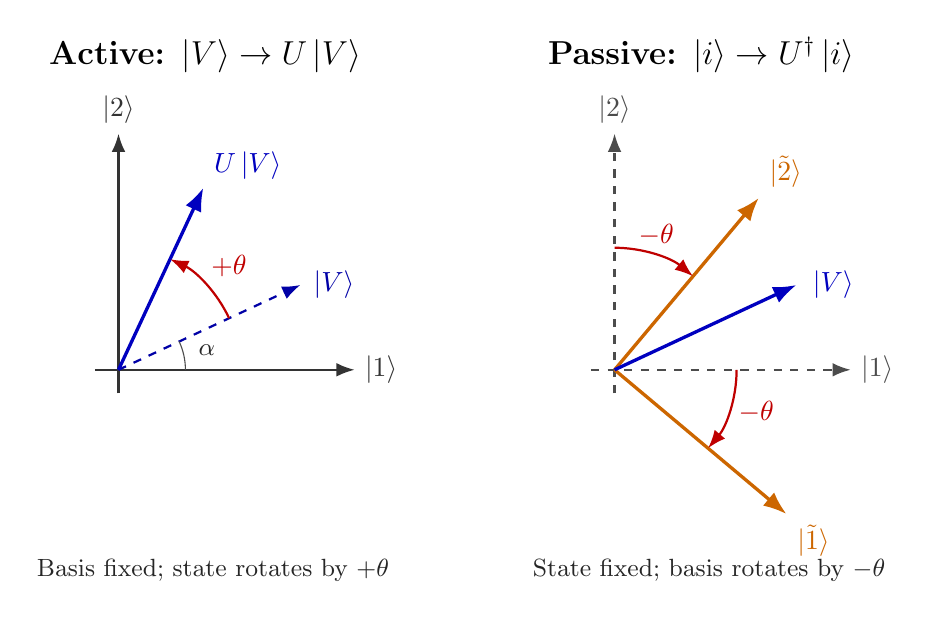
\begin{tikzpicture}[
    >=Latex,
    font=\normalsize,
    axis/.style={->, thick, black!80},
    oldaxis/.style={->, thick, dashed, black!70},
    newaxis/.style={->, very thick, orange!80!black},
    vec/.style={->, very thick, blue!75!black},
    oldvec/.style={->, thick, dashed, blue!65!black},
    rotarc/.style={->, thick, red!75!black}
]

% ================= Left Panel: Active Transformation =================
\begin{scope}[shift={(0,0)}]
    \node[font=\bfseries\large, anchor=south] at (1.1, 3.65) {Active: $\ket{V} \to U\ket{V}$};

    % Fixed basis axes
    \draw[axis] (-0.3, 0) -- (3.0, 0) node[right] {$\ket{1}$};
    \draw[axis] (0, -0.3) -- (0, 3.0) node[above] {$\ket{2}$};

    % Original vector at 25 deg
    \draw[oldvec] (0,0) -- (25:2.55) node[right, xshift=1pt] {$\ket{V}$};

    % Rotated vector at 65 deg
    \draw[vec] (0,0) -- (65:2.55) node[above right, yshift=-1pt] {$U\ket{V}$};

    % Rotation arc from 25 to 65
    \draw[rotarc] (25:1.55) arc (25:65:1.55) node[midway, above right, inner sep=2pt, red!75!black] {$+\theta$};

    % Angle alpha reference
    \draw[thin, black!70] (0:0.85) arc (0:25:0.85);
    \node[font=\small, black!85] at (12.5:1.15) {$\alpha$};

    \node[font=\small, black!85, align=center] at (1.2, -2.55) {Basis fixed; state rotates by $+\theta$};
\end{scope}

% ================= Right Panel: Passive Transformation =================
\begin{scope}[shift={(6.3,0)}]
    \node[font=\bfseries\large, anchor=south] at (1.1, 3.65) {Passive: $\ket{i} \to U^\dagger\ket{i}$};

    % Old basis axes (dashed)
    \draw[oldaxis] (-0.3, 0) -- (3.0, 0) node[right] {$\ket{1}$};
    \draw[oldaxis] (0, -0.3) -- (0, 3.0) node[above] {$\ket{2}$};

    % New basis axes rotated by -40 deg
    \draw[newaxis] (0,0) -- (-40:2.85) node[below right] {$\ket{\tilde{1}}$};
    \draw[newaxis] (0,0) -- (50:2.85) node[above right] {$\ket{\tilde{2}}$};

    % Fixed vector at 25 deg
    \draw[vec] (0,0) -- (25:2.55) node[right, xshift=2pt] {$\ket{V}$};

    % Rotation arcs for axes (-40 deg)
    \draw[rotarc] (0:1.55) arc (0:-40:1.55) node[midway, right, inner sep=3pt, red!75!black] {$-\theta$};
    \draw[rotarc] (90:1.55) arc (90:50:1.55) node[midway, above, inner sep=3pt, red!75!black] {$-\theta$};

    \node[font=\small, black!85, align=center] at (1.2, -2.55) {State fixed; basis rotates by $-\theta$};
\end{scope}

\end{tikzpicture}
\end{document}
